%package list
\documentclass{article}
\usepackage[top=3cm, bottom=3cm, outer=3cm, inner=3cm]{geometry}
\usepackage{multicol}
\usepackage{graphicx}
\usepackage{url}
%\usepackage{cite}
\usepackage{hyperref}
\usepackage{array}
%\usepackage{multicol}
\newcolumntype{x}[1]{>{\centering\arraybackslash\hspace{0pt}}p{#1}}
\usepackage{natbib}
\usepackage{pdfpages}
\usepackage{multirow}
\usepackage[normalem]{ulem}
\useunder{\uline}{\ul}{}
\usepackage{svg}
\usepackage{xcolor}
\usepackage{listings}
\lstdefinestyle{ascii-tree}{
    literate={├}{|}1 {─}{--}1 {└}{+}1 
  }
\lstset{basicstyle=\ttfamily,
  showstringspaces=false,
  commentstyle=\color{red},
  keywordstyle=\color{blue}
}
%\usepackage{booktabs}
\usepackage{caption}
\usepackage{subcaption}
\usepackage{float}
\usepackage{array}

\newcolumntype{M}[1]{>{\centering\arraybackslash}m{#1}}
\newcolumntype{N}{@{}m{0pt}@{}}


%%%%%%%%%%%%%%%%%%%%%%%%%%%%%%%%%%%%%%%%%%%%%%%%%%%%%%%%%%%%%%%%%%%%%%%%%%%%
%%%%%%%%%%%%%%%%%%%%%%%%%%%%%%%%%%%%%%%%%%%%%%%%%%%%%%%%%%%%%%%%%%%%%%%%%%%%
\newcommand{\itemEmail}{mvelasquea@unsa.edu.pe}
\newcommand{\itemStudent}{Mikhail Gabino Velasque Arcos}
\newcommand{\itemCourse}{Laboratorio FUNDAMENTOS DE LA PROGRAMACION II}
\newcommand{\itemCourseCode}{20214260}
\newcommand{\itemSemester}{II}
\newcommand{\itemUniversity}{Universidad Nacional de San Agustín de Arequipa}
\newcommand{\itemFaculty}{Facultad de Ingeniería de Producción y Servicios}
\newcommand{\itemDepartment}{Departamento Académico de Ingeniería de Sistemas e Informática}
\newcommand{\itemSchool}{Escuela Profesional de Ingeniería de Sistemas}
\newcommand{\itemAcademic}{2023 - B}
\newcommand{\itemInput}{Del 29 Setiembre 2023}
\newcommand{\itemOutput}{Al 3 Octubre 2023}
\newcommand{\itemPracticeNumber}{06}
\newcommand{\itemTheme}{ArreList}
%%%%%%%%%%%%%%%%%%%%%%%%%%%%%%%%%%%%%%%%%%%%%%%%%%%%%%%%%%%%%%%%%%%%%%%%%%%%
%%%%%%%%%%%%%%%%%%%%%%%%%%%%%%%%%%%%%%%%%%%%%%%%%%%%%%%%%%%%%%%%%%%%%%%%%%%%

\usepackage[english,spanish]{babel}
\usepackage[utf8]{inputenc}
\AtBeginDocument{\selectlanguage{spanish}}
\renewcommand{\figurename}{Figura}
\renewcommand{\refname}{Referencias}
\renewcommand{\tablename}{Tabla} %esto no funciona cuando se usa babel
\AtBeginDocument{%
	\renewcommand\tablename{Tabla}
}

\usepackage{fancyhdr}
\pagestyle{fancy}
\fancyhf{}
\setlength{\headheight}{30pt}
\renewcommand{\headrulewidth}{1pt}
\renewcommand{\footrulewidth}{1pt}
\fancyhead[L]{\raisebox{-0.2\height}{
\includegraphics[width=3cm]{img/logo_episunsa.png}}}
\fancyhead[C]{\fontsize{7}{7}\selectfont	\itemUniversity \\ \itemFaculty \\ \itemDepartment \\ \itemSchool \\ \textbf{\itemCourse}}
\fancyhead[R]{\raisebox{-0.2\height}{
\includegraphics[width=1.2cm]{img/logo_abet}}}
\fancyfoot[L]{Estudiante Mikhail Gabino Velasque Arcos}
\fancyfoot[C]{\itemCourse}
\fancyfoot[R]{Página \thepage}

% para el codigo fuente
\usepackage{listings}
\usepackage{color, colortbl}
\definecolor{dkgreen}{rgb}{0,0.6,0}
\definecolor{gray}{rgb}{0.5,0.5,0.5}
\definecolor{mauve}{rgb}{0.58,0,0.82}
\definecolor{codebackground}{rgb}{0.95, 0.95, 0.92}
\definecolor{tablebackground}{rgb}{0.8, 0, 0}

\lstset{frame=tb,
	language=bash,
	aboveskip=3mm,
	belowskip=3mm,
	showstringspaces=false,
	columns=flexible,
	basicstyle={\small\ttfamily},
	numbers=none,
	numberstyle=\tiny\color{gray},
	keywordstyle=\color{blue},
	commentstyle=\color{dkgreen},
	stringstyle=\color{mauve},
	breaklines=true,
	breakatwhitespace=true,
	tabsize=3,
	backgroundcolor= \color{codebackground},
}

\begin{document}
	
	\vspace*{10px}
	
	\begin{center}	
		\fontsize{17}{17} \textbf{ Informe de Laboratorio 06 }
	\end{center}
	\centerline{\textbf{\Large Tema: Arraylist}}
	%\vspace*{0.5cm}	

	\begin{flushright}
		\begin{tabular}{|M{2.5cm}|N|}
			\hline 
			\rowcolor{tablebackground}
			\color{white} \textbf{Nota}  \\
			\hline 
			     \\[30pt]
			\hline 			
		\end{tabular}
	\end{flushright}	

	\begin{table}[H]
		\begin{tabular}{|x{4.7cm}|x{4.8cm}|x{4.8cm}|}
			\hline 
			\rowcolor{tablebackground}
			\color{white} \textbf{Estudiante} & \color{white}\textbf{Escuela}  & \color{white}\textbf{Asignatura}   \\
			\hline 
			{\itemStudent \par \itemEmail} & \itemSchool & {\itemCourse \par Semestre: \itemSemester \par Código: \itemCourseCode}     \\
			\hline 			
		\end{tabular}
	\end{table}		
	
	\begin{table}[H]
		\begin{tabular}{|x{4.7cm}|x{4.8cm}|x{4.8cm}|}
			\hline 
			\rowcolor{tablebackground}
			\color{white}\textbf{Laboratorio} & \color{white}\textbf{Tema}  & \color{white}\textbf{Duración}   \\
			\hline 
			\itemPracticeNumber & \itemTheme & 04 horas   \\
			\hline 
		\end{tabular}
	\end{table}
	
	\begin{table}[H]
		\begin{tabular}{|x{4.7cm}|x{4.8cm}|x{4.8cm}|}
			\hline 
			\rowcolor{tablebackground}
			\color{white}\textbf{Semestre académico} & \color{white}\textbf{Fecha de inicio}  & \color{white}\textbf{Fecha de entrega}   \\
			\hline 
			\itemAcademic & \itemInput &  \itemOutput  \\
			\hline 
		\end{tabular}
	\end{table}
	
	\section{Actividades}
	\begin{itemize}		
		\item Cree un Proyecto llamado Laboratorio6
		\item Usted deberá crear las dos clases Soldado.java y VideoJuego3.java. Puede reutilizar lo
desarrollado en Laboratorios anteriores.
		\item Del Soldado nos importa el nombre, puntos de vida, fila y columna (posición en el tablero).
		
\item El juego se desarrollará en el mismo tablero de los laboratorios anteriores. Pero ahora el
tablero debe ser un ArrayList bidimensional.
\item Tendrá 2 Ejércitos. Inicializar el tablero con n soldados aleatorios entre 1 y 10 para cada
Ejército. Cada soldado tendrá un nombre autogenerado: Soldado0X1, Soldado1X1, etc., un
valor de puntos de vida autogenerado aleatoriamente [1..5], la fila y columna también
autogenerados aleatoriamente (no puede haber 2 soldados en el mismo cuadrado). Se debe
mostrar el tablero con todos los soldados creados (distinguir los de un ejército de los del otro
ejército). Además de los datos del Soldado con mayor vida de cada ejército, el promedio de
puntos de vida de todos los soldados creados por ejército, los datos de todos los soldados por
ejército en el orden que fueron creados y un ranking de poder de todos los soldados creados
por ejército (del que tiene más nivel de vida al que tiene menos) usando 2 diferentes
algoritmos de ordenamiento. Finalmente, que muestre qué ejército ganará la batalla (indicar
la métrica usada para decidir al ganador de la batalla).

	
	\end{itemize}
		
	\section{SOLUCIONARIO}
	\begin{itemize}
		\item Se hace el uso de arraylist  complementando lo avanzando anteriormente
	\end{itemize}

	\subsection{CODIGO FUENTE}
	\begin{itemize}	
		\item Se crea la clase soldado.java
		\item Se crea la clase principal:   VideJuego_v3.java
	\end{itemize}	
		
	\begin{lstlisting}[language=bash,caption={Creando la clase soldado y la clase VideoJuego_v3}][H]
		vim soldado.java
		  vim VideoJuego_v3.java
	\end{lstlisting}
	
	\begin{lstlisting}[language=bash,caption={Creando la clase Soldado}][H]
			
	public class Soldado {
		/*
		 Reusando el codiogo de los anterioes labs
		
			 laboratorio Nro 6 ejercicio 1
			 //clase soldado
			 Autor :Mikhail Gabino Velasque Arcos
			colaboro:---
			tiempo:
			 */
	   private String nombre;
	    private int puntosDeVida;
	    private int fila;
	    private int columna;

	    public Soldado(String nombre, int puntosDeVida) {
	        this.nombre = nombre;
	        this.puntosDeVida = puntosDeVida;
	    }

	    public String getNombre() {
	        return nombre;
	    }

	    public int getPuntosDeVida() {
	        return puntosDeVida;
	    }

	    public void setPuntosDeVida(int puntosDeVida) {
	        this.puntosDeVida = puntosDeVida;
	    }

	    public int getFila() {
	        return fila;
	    }

	    public void setFila(int fila) {
	        this.fila = fila;
	    }

	    public int getColumna() {
	        return columna;
	    }

	    public void setColumna(int columna) {
	        this.columna = columna;
	    }

	    @Override
	    public String toString() {
	        return "Nombre: " + nombre + ", Vida: " + puntosDeVida + ", Fila: " + fila + ", Columna: " + columna;
	    }
	}

			
			
			
			
			
	\end{lstlisting}	
	\begin{lstlisting}[language=bash,caption={Creando la clase principal de VideoJuego_v3.java}][H]
	
	public class VideoJuego_v3 {
	/*
	 Reusando el codiogo de los anterioes labs
	
		 laboratorio Nro 6 ejercicio 2
		 //clase soldado
		 Autor :Mikhail Gabino Velasque Arcos
		colaboro:---
		tiempo:
		 */

	 public static void main(String[] args) {
	        int filas = 10; 
	        int columnas = 10; 
	        int n = new Random().nextInt(10) + 1; 
	        ArrayList<Soldado> ejercito1 = crearEjercito(n, filas, columnas, "E1");
	        ArrayList<Soldado> ejercito2 = crearEjercito(n, filas, columnas, "E2");

	        mostrarTablero(filas, columnas, ejercito1, ejercito2);

	        System.out.println("\nEjército 1:");
	        mostrarEstadisticas(ejercito1);

	        System.out.println("\nEjército 2:");
	        mostrarEstadisticas(ejercito2);

	        String ganador = determinarGanador(ejercito1, ejercito2);
	        System.out.println("\nEl ejército ganador es: " + ganador);
	    }

	    public static ArrayList<Soldado> crearEjercito(int n, int filas, int columnas, String ejercitoPrefix) {
	        ArrayList<Soldado> ejercito = new ArrayList<>();
	        Random rand = new Random();
	        for (int i = 1; i <= n; i++) {
	            String nombre = ejercitoPrefix + "-" + i; 
	            int puntosDeVida = rand.nextInt(5) + 1; 

	            int fila, columna;
	            do {
	                fila = rand.nextInt(filas) + 1;
	                columna = rand.nextInt(columnas) + 1;
	            } while (yaOcupada(fila, columna, ejercito));
	            Soldado soldado = new Soldado(nombre, puntosDeVida);
	            soldado.setFila(fila);
	            soldado.setColumna(columna);
	            ejercito.add(soldado);
	        }
	        return ejercito;
	    }

	    public static boolean yaOcupada(int fila, int columna, ArrayList<Soldado> ejercito) {
	        for (Soldado soldado : ejercito) {
	            if (soldado.getFila() == fila && soldado.getColumna() == columna) {
	                return true;
	            }}
	        return false;
	    }
	    public static void mostrarTablero(int filas, int columnas, ArrayList<Soldado> ejercito1, ArrayList<Soldado> ejercito2) {
	        for (int fila = 1; fila <= filas; fila++) {
	            for (int columna = 1; columna <= columnas; columna++) { 
	                Soldado soldado1 = encontrarSoldadoEnPosicion(fila, columna, ejercito1);
	                Soldado soldado2 = encontrarSoldadoEnPosicion(fila, columna, ejercito2);
	                if (soldado1 != null) {
	                    System.out.print("|" + soldado1.getNombre() + "|");
	                } else if (soldado2 != null) {
	                    System.out.print("|" + soldado2.getNombre() + "|");
	                } else {
	                    System.out.print("|____|");
	                }}
	            System.out.println(); 
	        }}
	    public static Soldado encontrarSoldadoEnPosicion(int fila, int columna, ArrayList<Soldado> ejercito) {
	        for (Soldado soldado : ejercito) {
	            if (soldado.getFila() == fila && soldado.getColumna() == columna) {
	                return soldado;
	            }}
	        return null;
	    }
	    public static void mostrarEstadisticas(ArrayList<Soldado> ejercito) {
	        int totalVida = 0;
	        Soldado maxVida = ejercito.get(0);

	        for (Soldado soldado : ejercito) {
	            totalVida += soldado.getPuntosDeVida();
	            if (soldado.getPuntosDeVida() > maxVida.getPuntosDeVida()) {
	                maxVida = soldado;
	            }
	        }

	        System.out.println("Puntos de vida promedio: " + (double) totalVida / ejercito.size());
	        System.out.println("Soldado con mayor vida: " + maxVida);

	        System.out.println("\nLista de Soldados:");
	        for (Soldado soldado : ejercito) {
	            System.out.println(soldado);
	        }

	        System.out.println("\nRanking de poder:");
	        ordenarSoldadosPorPoder(ejercito);
	        for (Soldado soldado : ejercito) {
	            System.out.println(soldado);
	        }
	    }

	    public static void ordenarSoldadosPorPoder(ArrayList<Soldado> ejercito) {
	        Collections.sort(ejercito, new Comparator<Soldado>() {     
	            public int compare(Soldado s1, Soldado s2) {
	                return s2.getPuntosDeVida() - s1.getPuntosDeVida();
	            }
	        }
	        );
	    }
	    public static String determinarGanador(ArrayList<Soldado> ejercito1, ArrayList<Soldado> ejercito2) {
	        int totalVidaEjercito1 = calcularTotalVida(ejercito1);
	        int totalVidaEjercito2 = calcularTotalVida(ejercito2);
	        if (totalVidaEjercito1 > totalVidaEjercito2) {
	            return "Ejército 1 (E1)";
	        } else if (totalVidaEjercito1 < totalVidaEjercito2) {
	            return "Ejército 2 (E2)";
	        } else {
	            return "Empate";
	        }}
	    public static int calcularTotalVida(ArrayList<Soldado> ejercito) {
	        int totalVida = 0;
	        for (Soldado soldado : ejercito) {
	            totalVida += soldado.getPuntosDeVida();
	        }
	        return totalVida;
	    }
	}
	
	
	
	
				\end{lstlisting}
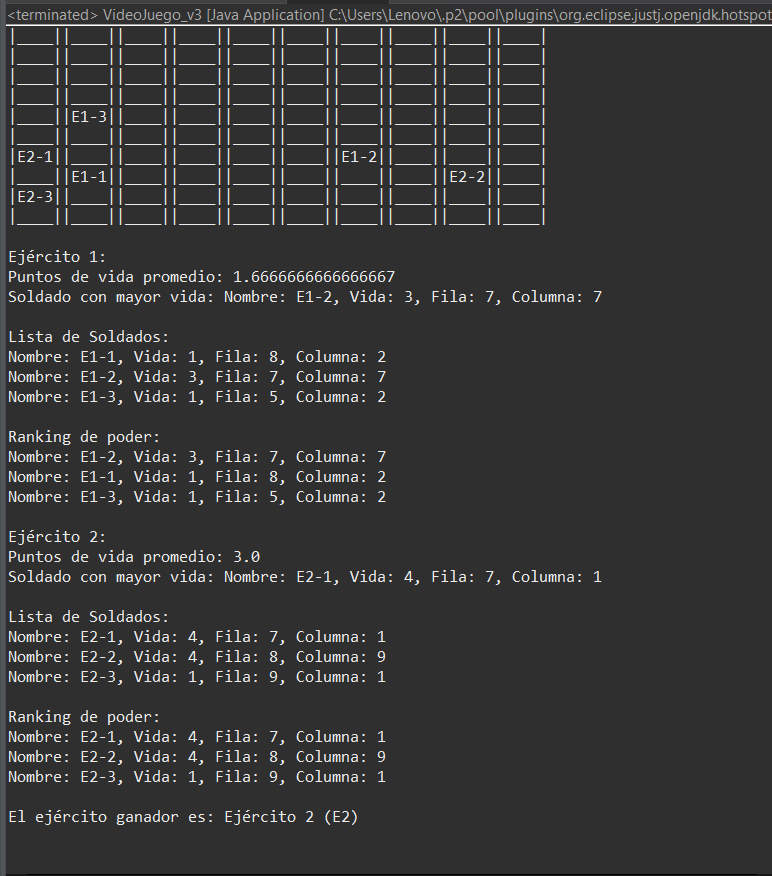
\includegraphics[scale=1]{../../Proyecto/fp2-23b/fase01/lab06/latex/img/imagen.png} 		
\end{document}